
\documentclass[tikz,border=2mm]{standalone}
\usepackage[utf8]{inputenc}
\usepackage[T1]{fontenc}
\usepackage{amsmath}
\usepackage{amssymb}
\usetikzlibrary{arrows.meta,positioning,calc,shapes.geometric}
\usepackage{xcolor}

\definecolor{inkNavy}{HTML}{1B2733}
\definecolor{slate}{HTML}{3B4B5C}
\definecolor{paper}{HTML}{FBFAF7}
\definecolor{amber}{HTML}{C97A2B}
\definecolor{teal}{HTML}{2E7D74}
\definecolor{softred}{HTML}{A6402F}
\definecolor{lightgrey}{HTML}{E7E4DD}
\definecolor{midgrey}{HTML}{8B8A85}

\begin{document}
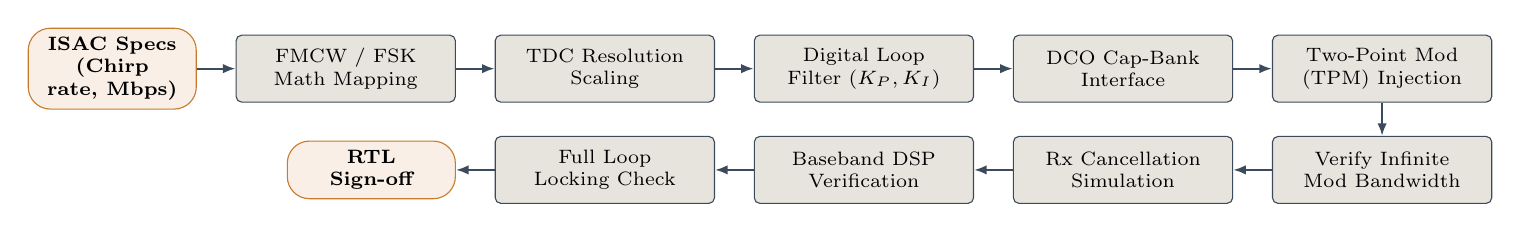
\begin{tikzpicture}[
  node distance=6pt and 14pt,
  box/.style={draw=slate, fill=lightgrey, rounded corners=2pt, text width=2.55cm, align=center, minimum height=0.85cm, font=\scriptsize},
  term/.style={draw=amber, fill=amber!12, rounded corners=8pt, text width=1.9cm, align=center, minimum height=0.7cm, font=\scriptsize\bfseries},
  arr/.style={-{Latex[length=1.6mm]}, slate, thick}
]
\node[term] (spec) {ISAC Specs\\(Chirp rate, Mbps)};
\node[box, right=of spec] (wave) {FMCW / FSK\\Math Mapping};
\node[box, right=of wave] (tdc) {TDC Resolution\\Scaling};
\node[box, right=of tdc] (dlf) {Digital Loop\\Filter ($K_P, K_I$)};
\node[box, right=of dlf] (dco) {DCO Cap-Bank\\Interface};
\node[box, right=of dco] (tpm) {Two-Point Mod\\(TPM) Injection};

\node[box, below=12pt of tpm] (band) {Verify Infinite\\Mod Bandwidth};
\node[box, left=of band] (canc) {Rx Cancellation\\Simulation};
\node[box, left=of canc] (dsp) {Baseband DSP\\Verification};
\node[box, left=of dsp] (pvt) {Full Loop\\Locking Check};
\node[term, left=of pvt] (fin) {RTL\\Sign-off};

\draw[arr] (spec)--(wave); \draw[arr] (wave)--(tdc); \draw[arr] (tdc)--(dlf);
\draw[arr] (dlf)--(dco); \draw[arr] (dco)--(tpm); \draw[arr] (tpm)--(band);
\draw[arr] (band)--(canc); \draw[arr] (canc)--(dsp); \draw[arr] (dsp)--(pvt);
\draw[arr] (pvt)--(fin);
\end{tikzpicture}
\end{document}